%%%%%%%%%%%%%%%%%%%%%%%%%%%%%%%%%%%%%%%%%%%%%%%%%%%%%%%%%%%%%%%%%%%%%%
%%                     Stimulation
%%%%%%%%%%%%%%%%%%%%%%%%%%%%%%%%%%%%%%%%%%%%%%%%%%%%%%%%%%%%%%%%%%%%%%

\subsubsection{Glyph: \glyph{Stimulation}}\label{sec:stimulation}
%\color{blue}

A \glyph{stimulation} affects \textbf{positively} the strength, or the probability, of the target relationship. This stimulation can be for instance a catalysis or a positive allosteric regulation.

\begin{glyphDescription}
 \glyphSboTerm SBO:0000170 ! stimulation.
 \glyphOrigin Any \glyph{entity node} (\sect{ENs}).
 \glyphTarget Any \glyph{relationship} (\sect{relationships}).
 \glyphEndPoint The target extremity of a \glyph{stimulation} carries an empty arrowhead.
 \glyphAux A \glyph{unit of information} carrying the mention \glyph{cis} or \glyph{trans} precises the relationship between the \glyph{entity node} from which the \glyph{stimulation} origins and either:
\begin{itemize}
\item the \glyph{entity node} from which the influence targeted by the \glyph{stimulation} origins
\item all the relevant \glyph{interactors} of the \glyph{interaction} or the \glyph{non-interaction} targeted by the \glyph{stimulation}
\item the \glyph{entity} subjected to the \glyph{assignment} targeted by the \glyph{stimulation}
\end{itemize}
 \end{glyphDescription}

\begin{figure}[H]
  \centering
  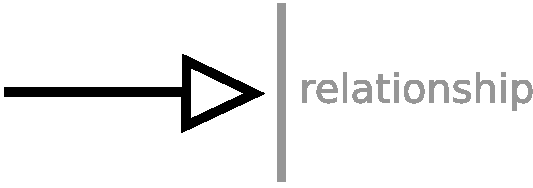
\includegraphics[scale = 0.5]{images/stimulation}
  \caption{The \ER glyph for \glyph{stimulation}.}
  \label{fig:stimulation}
\end{figure}

\begin{figure}[H]
  \centering
  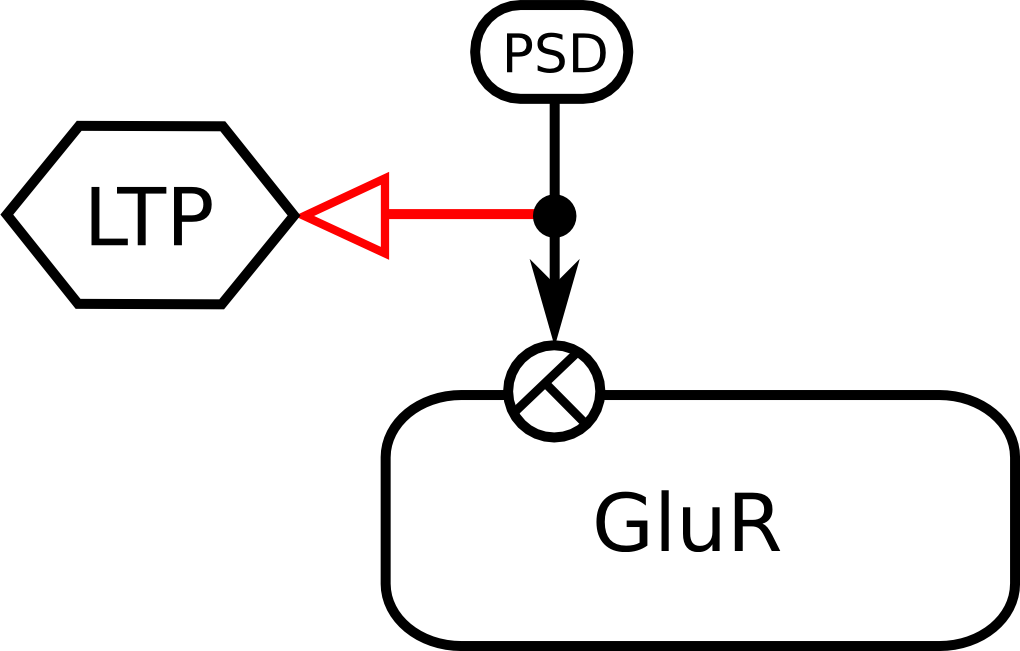
\includegraphics[scale = 0.5]{examples/ex-stimulation}
  \caption{Example of a \glyph{stimulation} a \glyph{phenotype} ``Long Term Potentiation (LTP)'' enhanced when the entity ``GluR'' is present in the post-synaptic density.}
  \label{fig:ex-stimulation}
\end{figure}

\normalcolor



